%%%%%%%%%%%%%%%%%%%%%%%%%%%%%%%%%%%%%%%%%
% Programming/Coding Assignment
% LaTeX Template
%
% This template has been downloaded from:
% http://www.latextemplates.com
%
% Original author:
% Ted Pavlic (http://www.tedpavlic.com)
%
% Note:
% The \lipsum[#] commands throughout this template generate dummy text
% to fill the template out. These commands should all be removed when 
% writing assignment content.
%
% This template uses a Perl script as an example snippet of code, most other
% languages are also usable. Configure them in the "CODE INCLUSION 
% CONFIGURATION" section.
%
%%%%%%%%%%%%%%%%%%%%%%%%%%%%%%%%%%%%%%%%%

%----------------------------------------------------------------------------------------
%	PACKAGES AND OTHER DOCUMENT CONFIGURATIONS
%----------------------------------------------------------------------------------------

\documentclass{article}

\usepackage{fancyhdr} % Required for custom headers
\usepackage{lastpage} % Required to determine the last page for the footer
\usepackage{extramarks} % Required for headers and footers
\usepackage[usenames,dvipsnames]{color} % Required for custom colors
\usepackage{graphicx} % Required to insert images
\usepackage{listings} % Required for insertion of code
\usepackage{courier} % Required for the courier font
\usepackage{subcaption}
\usepackage{url}

% Margins
\topmargin=-0.45in
\evensidemargin=0in
\oddsidemargin=0in
\textwidth=6.5in
\textheight=9.0in
\headsep=0.25in

\linespread{1.1} % Line spacing

% Set up the header and footer
\pagestyle{fancy}
\lhead{\hmwkAuthorName} % Top left header
\rhead{\firstxmark} % Top right header
\lfoot{\lastxmark} % Bottom left footer
\cfoot{} % Bottom center footer
\rfoot{Page\ \thepage\ of\ \protect\pageref{LastPage}} % Bottom right footer
\renewcommand\headrulewidth{0.4pt} % Size of the header rule
\renewcommand\footrulewidth{0.4pt} % Size of the footer rule

\setlength\parindent{0pt} % Removes all indentation from paragraphs

%----------------------------------------------------------------------------------------
%	CODE INCLUSION CONFIGURATION
%----------------------------------------------------------------------------------------

\definecolor{MyDarkGreen}{rgb}{0.0,0.4,0.0} % This is the color used for comments
\lstloadlanguages{C++}
\lstset{language=[11]C++,
        frame=single, % Single frame around code
        basicstyle=\small\ttfamily, % Use small true type font
        keywordstyle=[1]\color{Blue}\bf, % functions bold and blue
        keywordstyle=[2]\color{Purple}, % function arguments purple
        keywordstyle=[3]\color{Blue}\underbar, % Custom functions underlined and blue
        identifierstyle=, % Nothing special about identifiers                                         
        commentstyle=\usefont{T1}{pcr}{m}{sl}\color{MyDarkGreen}\small, % Comments small dark green courier font
        stringstyle=\color{Purple}, % Strings are purple
        showstringspaces=false, % Don't put marks in string spaces
        tabsize=4, % 4 spaces per tab
        morecomment=[l][\color{Blue}]{...}, % Line continuation (...) like blue comment
        numbers=left, % Line numbers on left
        firstnumber=1, % Line numbers start with line 1
        numberstyle=\tiny\color{Blue}, % Line numbers are blue and small
        stepnumber=5 % Line numbers go in steps of 5
}

%----------------------------------------------------------------------------------------
%	NAME AND CLASS SECTION
%----------------------------------------------------------------------------------------

\newcommand{\hmwkTitle}{Color histogram} % Assignment title
\newcommand{\hmwkDueDate}{Tuesday,\ February\ 28,\ 2017} % Due date
\newcommand{\hmwkClass}{BM40A1400 GPGPU course project} % Course/class
\newcommand{\hmwkAuthorName}{Maria Glukhova \& 500503 Ekaterina Nepovinnykh} % Your name

%----------------------------------------------------------------------------------------
%	TITLE PAGE
%----------------------------------------------------------------------------------------

\title{
\vspace{2in}
\textmd{\textbf{\hmwkClass:\ \hmwkTitle}}\\
\normalsize\vspace{0.1in}\small{Due\ on\ \hmwkDueDate}\\
\vspace{3in}
}

\author{\textbf{\hmwkAuthorName}}
\date{} % Insert date here if you want it to appear below your name

%----------------------------------------------------------------------------------------

\begin{document}

\maketitle

%----------------------------------------------------------------------------------------
%	TABLE OF CONTENTS
%----------------------------------------------------------------------------------------

%\setcounter{tocdepth}{1} % Uncomment this line if you don't want subsections listed in the ToC

\newpage
\tableofcontents
\newpage

\section{Introduction}
The goal of this project is to create a color histogram for provided image using
GPGPU and CUDA \cite{CUDA}.

This course project includes the following tasks:

\begin{enumerate}
\item GPU implementation of color histogram \cite{cudahist}
\item Multiple GPU support
\item CPU implementation for performance comparison
\item Matlab implementation to confirm that GPU implementation is faster
\item Python wrapper using PyCuda \cite{pycuda}
\end{enumerate}

The work was done in a public repository on GitHub (see \cite{gh}).

\section{CUDA Implementation}
CUDA-based computation of color histogram is performed in two steps:

\begin{enumerate}
\item Gather information into partial histograms using atomic counters
\item Accumulate partial histograms into one resulting histogram
\end{enumerate}

Both steps are performed as GPU kernels using one intermediate GPU memory buffer
and the result is then copied back into host memory.

\subsection{First-pass kernel}
Listing~\ref{lst:histogram_gmem_atomics} shows first-pass histogram kernel.
It gathers the information from a part of the image to the partial hisogram.
Part of the image is defined by block and grid size
("part of image" is not a continious patch here, rather every n-th pixel).
The partial histogram is stored in global memory defined by "out".
Every block has a group number (g) assigned to it, and it treats part of
global memory (from out + g * NUM\_PARTS and every nt bits, where nt is the size (x*y)
of the grid) as its own, storing the histogram of its part of the image here.

What happens in the kernel is:

the blocks' own bits of global memory get initialized with zeros.

Every corresponding (assigned to this block) pixel get visited, and:

\begin{enumerate}
\item Pixel is decoded into several (ACTIVE\_CHANNELS) colors.
\item These values are binned to the desired number of bins (NUM\_BINS).
\item Corresponding values in a partial histogram (part of global memory) get updated.
\end{enumerate}

Parts 1 and 2 are implemented in DecodePixel (see listing~\ref{lst:DecodePixel}).

\subsection{Accumulating partial histograms}
Listing~\ref{lst:histogram_gmem_accum} shows \textbf{histogram\_gmem\_accum} kernel
which gathers partial histograms from global memory (in) into output histogram.

Partial histograms are expected to be stored in a part of global memory of
n * ACTIVE\_CHANNELS * NUM\_BINS * sizeof(uint) size.
It is expected that every nth bit belongs to the same partial histogram
(the k-th histogram stored in k, n + k, 2 * n + k, ... elements).

Every block running the kernel has a particular bin on the output histogram it is
responsible for. It gathers information about this bin from every partial histogram,
and sums it up.

\subsection{CPU wrapper for kernel execution}
Listing~\ref{lst:run_gmem_atomics} shows a function \textbf{run\_gmem\_atomics}
which is a CPU wrapper for the histogram computation. It assigns the blocks,
allocates the memory for partial histograms, computes them using
\textbf{histogram\_gmem\_atomics} (see listing~\ref{lst:histogram_gmem_atomics})
and accumulates with \textbf{histogram\_gmem\_accum}
(see listing~\ref{lst:histogram_gmem_accum}).

\subsection{Multiple GPU support}
Multiple GPU version is implemented similarly to single GPU one, but with extra
parallelization based on color channel. As such, every device has a specific color
channel assigned to it. Listings \ref{lst:histogram_gmem_atomics1} and
\ref{lst:run_multigpu} show implementation of multi-GPU color histogram computation.

\section{Matlab implementation}
Listing~\ref{lst:matlab_hist} shows a matlab function that computes color histogram
of an input image. The function accepts the image itself, bit depth of an image and
the number of bins in the resulting histogram. The function performs the necessary
computation in exactly \(W*H*C\) consecutive steps, where:

\begin{description}
\item [W] is the width of an image in pixels
\item [H] is the height of an image in pixels
\item [C] is the number of color channels in an image
\end{description}

As such, among the images with the same number of color channels and the same color
depth this implementation is expected to take linear amount of time relative to
the total numer of pixels in an image.

\section{Python wrapper}
As a part of the task, python wrapper using exising C++-based CUDA code was
implemented. The relevant part of the wrapper is presented in
listing~\ref{lst:python_wrapper}. The algorithm is essentially the same as with C++
version, except Python wrapper requires convertion of native numeric types to their
numpy equivalent in order to preserve memory layout for GPU kernels.

\section{Experiments}
Experiments were conducted on LUT GPGPU cluster in order to determite runtime
characteristics of various implementations on the same set of images. The goal is
to assert that GPGPU implementation is faster on larger images than both C++ and
Matlab implementations. Another goal is to confirm that CPU implementation is linear
relative to total number of pixels in an image while GPU is sub-linear.

Fig.~\ref{fig:plasma0500}, fig.~\ref{fig:bstar100} and
fig.~\ref{fig:spotted_ball_3500} show examples of images that were used during testing.
Several image samples have been prepared with different sizes and color depths in
order to mesure performance of all implemented methods.

\begin{figure}
\centering
\begin{subfigure}[b]{0.3\textwidth}
        
\includegraphics[width=\textwidth]{../data/plasma0500.png}
        \caption{plasma0500.png test image (size: 500x500px)}
        \label{fig:plasma0500}
\end{subfigure}
~
\begin{subfigure}[b]{0.3\textwidth}
        
\includegraphics[width=\textwidth]{../data/spotted_ball_3500.png}
        \caption{spotted\_ball\_3500.png test image (size: 3500x3500px)}
        \label{fig:spotted_ball_3500}
\end{subfigure}
~
\begin{subfigure}[b]{0.3\textwidth}
        
\includegraphics[width=\textwidth]{../data/bstar100.png}
        \caption{bstar100.png test image (size: 100x100px)}
        \label{fig:bstar100}
\end{subfigure}
\caption{Test images}
\label{fig:test_images}
\end{figure}

Fig.~\ref{fig:run_plot} shows the plot that compares different implementations total run time relative
to size of an input image. The plot clearly shows that CPU-based implementations
have linear relative to total number of pixels while GPGPU-based implementations are
sub-linear. The best performance was achieved on single-GPU implementation, probably
due to syncronization between different devices on multi-GPU version.

\begin{figure}
\centering
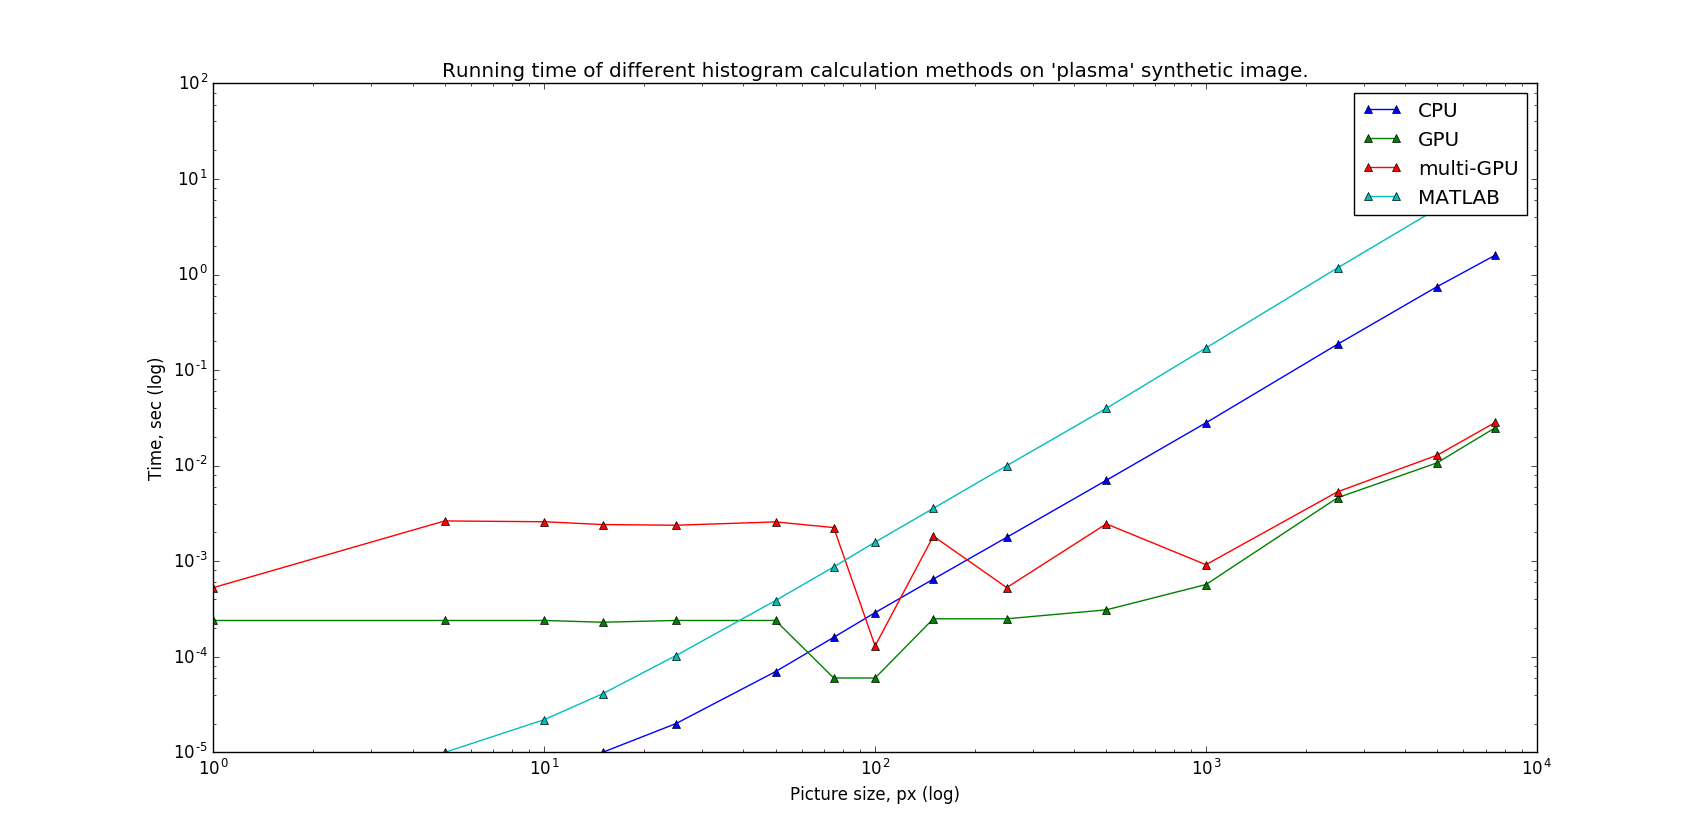
\includegraphics[width=\textwidth]{./figures/runtime_log_with_matlab.png}
\caption{Comparison of performance between different implementations of color histogram}
\label{fig:run_plot}
\end{figure}

% ----------------------------------------------------------------------------------
%                                  CODE LISTINGS
% ----------------------------------------------------------------------------------
\clearpage
\section{Code listings}
\lstinputlisting[
        caption=First-pass histogram kernel,
        label=lst:histogram_gmem_atomics,
        language=C++,
        firstline=51,
        lastline=100
]{../ColorHistograms-cuda/src/histogram_gpu.cu}
\lstinputlisting[
        caption=Decode uchar4 pixel into bins,
        label=lst:DecodePixel,
        language=C++,
        firstline=33,
        lastline=49
]{../ColorHistograms-cuda/src/histogram_gpu.cu}
\lstinputlisting[
        caption=Accumulate partial histograms into global one,
        label=lst:histogram_gmem_accum,
        language=C++,
        firstline=102,
        lastline=124
]{../ColorHistograms-cuda/src/histogram_gpu.cu}
\clearpage
\lstinputlisting[
        caption=CPU Wrapper for GPU histogram computation,
        label=lst:run_gmem_atomics,
        language=C++,
        firstline=126,
        lastline=165
]{../ColorHistograms-cuda/src/histogram_gpu.cu}
\clearpage
\lstinputlisting[
        caption=First pass histogram kernel for multiple GPUs,
        label=lst:histogram_gmem_atomics1,
        language=C++,
        firstline=168,
        lastline=212
]{../ColorHistograms-cuda/src/histogram_gpu.cu}
\clearpage
\lstinputlisting[
        caption=CPU Wrapper for multiple GPUs histogram computation,
        label=lst:run_multigpu,
        language=C++,
        firstline=215,
        lastline=254
]{../ColorHistograms-cuda/src/histogram_gpu.cu}
\clearpage
\lstinputlisting[
        caption=Matlab function for computing color histogram of an image,
        label=lst:matlab_hist,
        language=Matlab,
        firstline=1,
        lastline=27
]{../ColorHistograms-matlab/histogram.m}
\lstinputlisting[
        caption=Python wrapper that runs CUDA-based color histogram calculation,
        label=lst:python_wrapper,
        language=Python,
        firstline=7,
        lastline=27
]{../ColorHistograms-python/color_histogram_cuda.py}

\clearpage
\bibliographystyle{unsrt}
\bibliography{report.bib}
\end{document}